\chapter{ПРОЕКТИРОВАНИЕ СИСТЕМЫ УПРАВЛЕНИЯ ДВИЖЕНИЕМ БЕСПИЛОТНОГО АВТОМОБИЛЯ}
В данной главе рассматривается этап проектирования структуры и алгоритмов системы управления движением беспилотного
автомобиля. Проектирование системы основано на анализе рассмотренных архитектурных решений и алгоритмов.

\section{Формулирование требований к разрабатываемой системе}


Система управления беспилотным автомобилем должна выполнять большое количество функций, необходимых для эффективного
и безопасного движения в сложных условиях, среди которых
\begin{itemize}
    \item распознавание других участников дорожного движения (автомобилей, пешеходов,
          велосипедистов и т.п.);
    \item отслеживать других участников дорожного движения в течении некоторого времени для определения характеристик
          их движения и уменьшения ошибок распознавания;
    \item определять положение, скорость, ускорение и предсказывать будущие действия других участников дорожного
          движения;
    \item распознавать дорожные знаки, светофоры;
    \item распознавать дорожную разметку;
    \item на основании всей собранной информации осуществлять планирование безопасного и эффективного движения;
    \item выполнять запланированное движение и реагировать на изменения в дорожной ситуации.
\end{itemize}

Исходя из требуемой функциональности, а так же критериев безопасности, система управления беспилотным автомобилем
обладает высочайшей сложностью. Разработку такой системы невозможно осуществить в полной мере сразу, по "водопадной"
модели. Различные компоненты системы должны разрабатываться и улучшаться независимо, чтобы наращивать функциональность
и увеличивать безопасность и эффективность системы управления.

Поэтому главным требованием к системе управления беспилотным автомобилем является высокая модульность, что позволит
разрабатывать и тестировать отдельные системы и подсистемы независимо.

Другим требованием, также приводящим к необходимости модульной системы, является необходимость иметь возможность
тестирования компонентов системы управления беспилотным автомобилем на небольших моделях и с использованием различных
симуляторов и иных средств моделирования, что позволит быстрее приступить
к разработке системы, не завися от реализации системы управления органами управления реального автомобиля.

В связи с очень большим объемом работ, требуемом для разработки полной системы управления беспилотного автомобиля, в
рамках данной работы будет осуществляться разработка небольшой части требуемой функциональности:
\begin{itemize}
    \item осуществление движения по заданной траектории с обратной связью;
    \item осуществление локального планирования, чтобы формировать оптимальные или близкие к ним траектории движения,
          позволяющие достичь поставленной локальной цели;
    \item прототип системы распознавание препятствий, способный распознавать простейшие статические препятствия,
          для того, чтобы экспериментально проверить предыдущие две возможности;
    \item управление исполнительными органами мобильной платформы для выполнения запланированных движений.
\end{itemize}

\section{Проектирование общей архитектуры системы управления движением}

Разрабатываемую в рамках данной работы систему управления можно разделить на несколько частей: драйвер автомобиля,
система распознавания препятствий, система планирования локальной траектории и система следования по траектории.

Для отработки и тестирования системы управления необходимо построить небольшую мобильную платформу, которая будет
использоваться для проведения экспериментов. Мобильная платформа должна быть оснащена датчиками, используемыми для
распознавания препятствий и определения собственного положения в локальной системе координат, необходимого для
реализации движения по траектории с обратной связью. Платформа должна быть оснащена встраиваемым компьютером достаточной
производительности. Помимо этого, разумеется, необходимо осуществлять управление приводами платформы.

Для осуществления управления беспилотным автомобилем необходим ряд сенсоров, обеспечивающих систему управления
необходимой информацией об окружающей обстановке. Беспилотные автомобили, разрабатываемые крупными компаниями
оснащены множество сенсоров, описанных в первой главе. Основными типами сенсоров являются камеры, LiDAR, радары,
GPS и другие.

Система компьютерного зрения является одним из самых сложных и критичных компонентов системы управления беспилотного
автомобиля, от надежности и работы которой зависит безопасность автомобиля и других участников дорожного движения.
Разработка системы компьютерного зрения, которая в полной мере удовлетворяет этим требованиям ~--- крайне сложная и
ресурсоемкая задача, над решением которой в течении многих лет работают ведущие компании-разработчики беспилотных
автомобилей и, тем не менее, эта задача далека от полного решения.

Все современные, start-of-the-art, системы компьютерного зрения используют глубокие нейронные сети для решения таких
задач, как детектирование объектов, детектирование дороги (области доступной для движения), детектирования дорожной
разметки, детектирования светофоров и дорожных знаков, предсказания намерений других участников движения. В этих задачах
глубокие нейронные сети давно являются стандартом де-факто и существенно превосходят по точности распознавания любые
классические алгоритмы. Тем не менее, использование технологий машинного обучения, в частности, глубоких нейронных
сетей, приводит к дополнительным трудностям. Помимо разработки архитектуры нейронной сети, поиска ее параметров, крайне
важную роль играют данные, используемые для обучения нейронной сети. Именно данные играют критическую роль в том, как
система компьютерного зрения будет выполнять свою работу, особенно в сложных условиях и редких ситуациях. Добиться
правильного поведения нейросетевого алгоритма в тех ситуациях, когда он ошибается, можно только с помощью предоставления
дополнительных обучающих данных, покрывающих этот случай. Крупные компании, обладающие доступом к огромным массивом
данных имеют значительное преимущество в этой области. Так, например, компания Tesla, располагает парком из сотен
тысяч автомобилей, которые предоставляют телеметрию, позволяя определять ситуации, в которых работа автопилота была
некорректна, собирать похожие ситуации, записанные автомобилями по всему миру, и оперативно дообучать используемые
нейронные сети.

В связи с высокой сложностью разработки системы компьютерного зрения, в данной работе не рассматривается разработка
полноценной системы компьютерного зрения. Тем не менее, с целью отладки алгоритмов планирования движения и движения
по траектории, необходимо разработать простую систему компьютерного зрения, которая бы решала следующи задачи:
\begin{itemize}
      \item определение положения и ориентации модели автомобиля с точностью, достаточной для работы регулятора с
            обратной связью ддя точного движения по траектории;
      \item определение статических препятствий, с целью проверки системы объезда препятствий.
\end{itemize}

Для реализации первой задачи было решено применять алгоритм одновременной картографии и навигации (SLAM) на основе
стереозрения. SLAM-алгоритмы не позволяют получать глобальное положение автомобиля и подвержены накоплению ошибок при
передвижении на большие расстояния, но для проверки задачи локального планирования движения они хорошо подходят, потому
что обеспечивают высокую точность позиционирования и частоту обновления данных.

Для определения препятствий было решено использовать шестнадцатилучевой LiDAR Velodyne VLP-16, который был приобретен
для проекта беспилотного автомобиля и предполагался для установки на полноразмерный автомобиль. LiDAR позволяет получить
трехмерное облако точек, представляющее окружающую обстановку, обладающее сравнительно большой детализацией, обнаруживая
препятствия на расстояниях до ста метров. Использование LiDAR для малой мобильной платформы кажется избыточным, но
качественное облако точек, которое он предоставляет, существенно облегчает задачу обнаружения препятствий.

Диаграмма компонентов системы управления беспилотным автомобилем представлена на рисунке
\ref{img:system_component_diagram}. Все компоненты можно разделить на следующие группы:
\begin{itemize}
      \item драйверы сенсоров, осуществляющие работу с сенсорами, такими как LiDAR и камеры, и предоставляющие
            API для удобного получения данных другими компонентам системы управления;
      \item основные компоненты системы управления, осуществляющие основную работу по восприятию окружающей
            обстановки, планированию и управлению движением;
      \item драйверы исполнительных устройств автомобиля, позволяющие исполнять сформированные последовательности
            команд непосредственно аппаратным оборудованием автомобиля.
\end{itemize}

\begin{figure}[h]
      \centering
      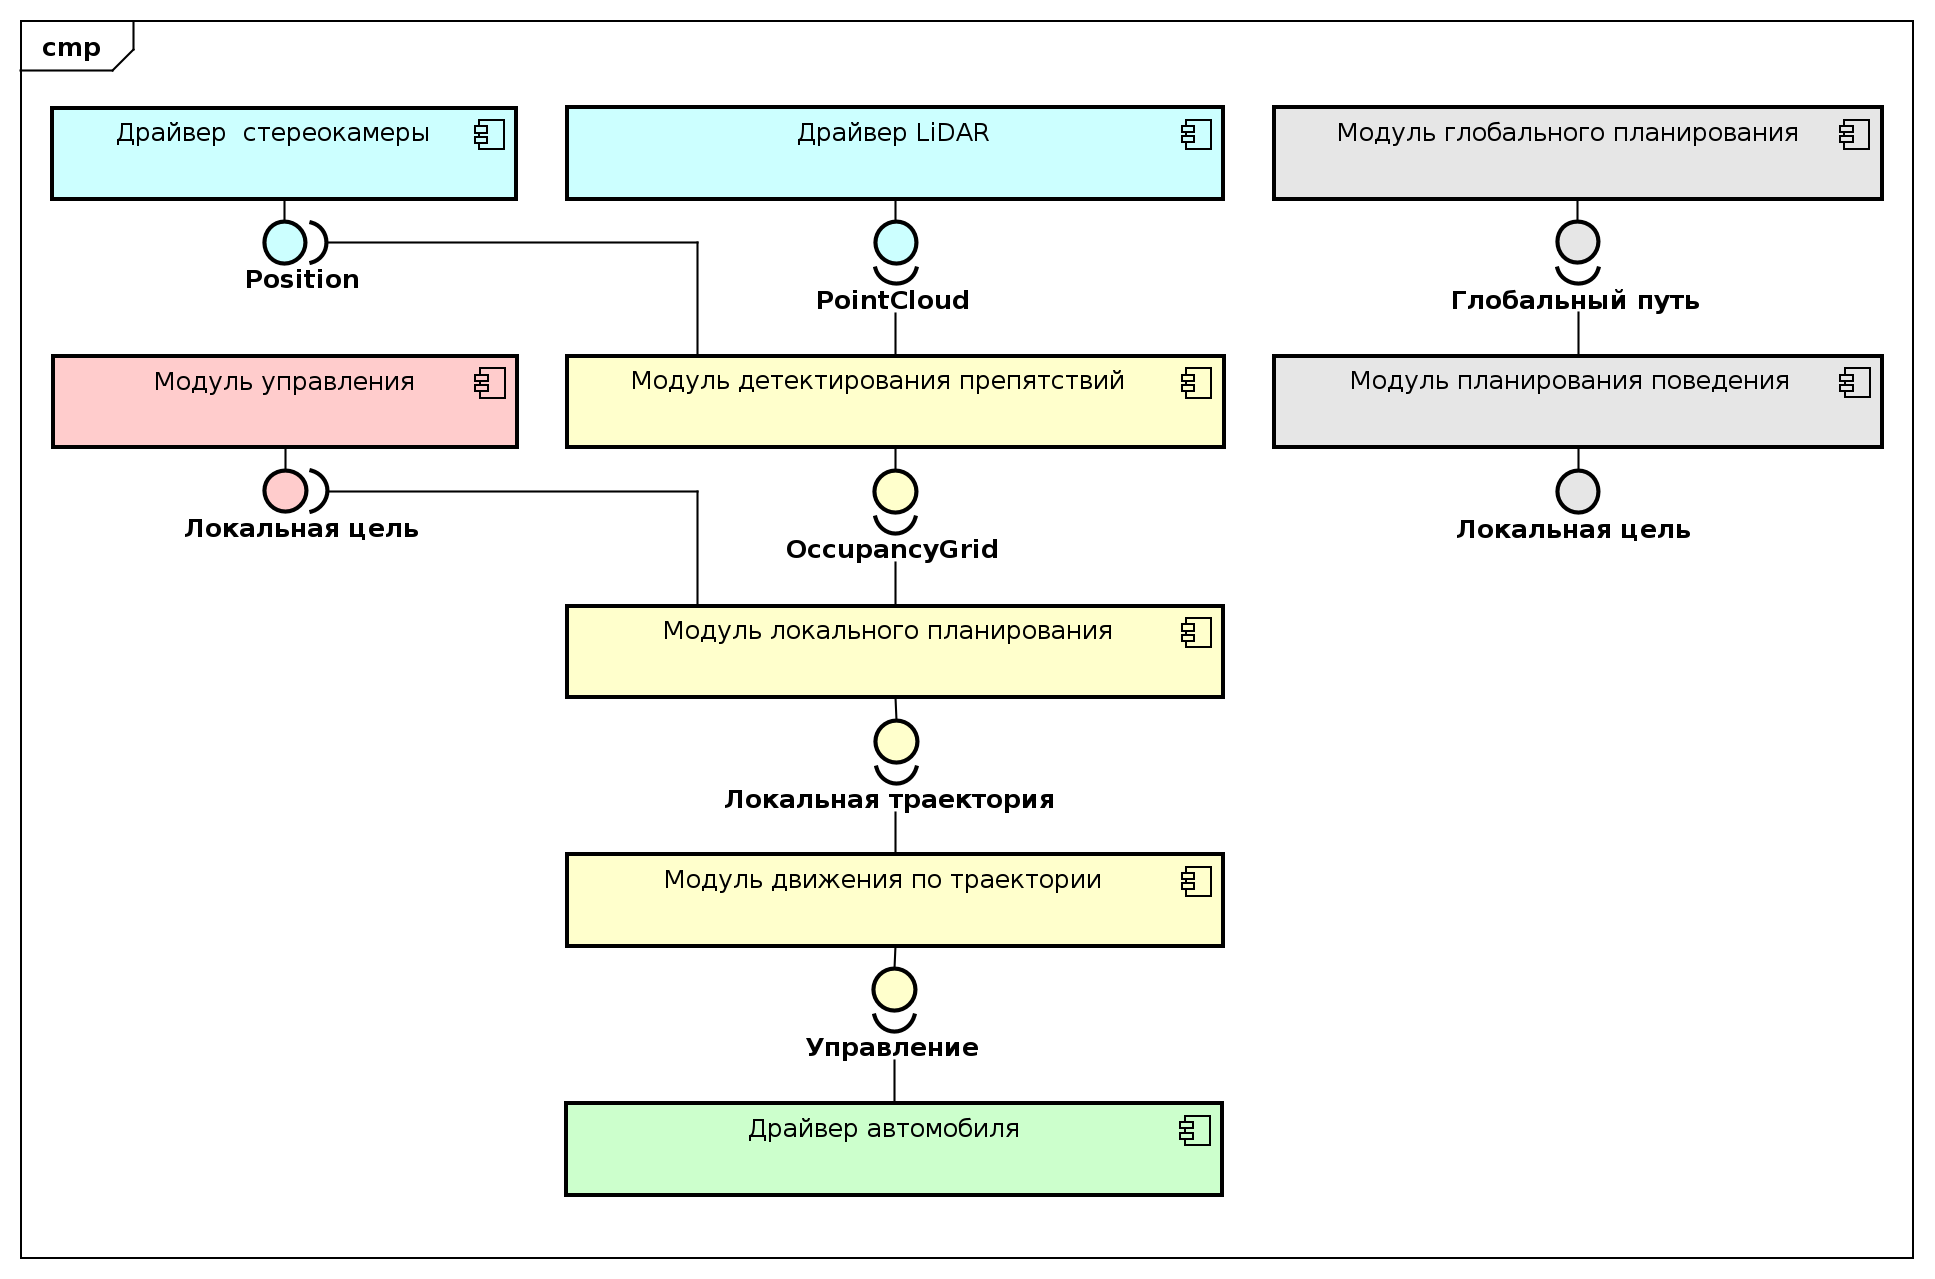
\includegraphics[width=\linewidth]{images/system_component_diagram}
      \caption{Диаграмма компонентов системы управления беспилотным автомобилем}
      \label{img:system_component_diagram}
  \end{figure}

Драйвер стереокамеры реализует работу со стереокамерой и алгоритм SLAM. Этот модуль предоставляет данные о текущем
положении и ориентации автомобиля в локальной системе координат. Драйвер LiDAR предоставляет облако точек, полученное
с LiDAR. Модуль детектирования препятствий осуществляет базовое детектирование препятствий в полученном облаке точек
и представляет информацию о них в виде т.н. Occupancy Grid. Occupancy Grid - это распространенный способ представления
информации о препятствиях в виде регулярной двухмерной сетки, каждая ячейка которой может быть в одном из трех
состояний: свободно, препятствие или неизвестно. Система управления беспилотным автомобилем в общем виде имеет модули
глобального планирования и планирования поведения, которые отвечают за построение глобальной траектории по дорожной
сети и принятие решений в соответствии с окружающей обстановкой и правилами дорожного движения, как было рассмотрено
в первой главе \ref{img:general_arch}. В рамках данной работы эти модули не рассматриваются и заменяются пользовательским
интерфейсом оператора, с помощью которого можно вручную указать локальную цель, вместо того, чтобы она задавалась
планировщиком поведения. На основании локальной цели, текущего положения автомобиля, полученного от модуля SLAM, и
инофрмации о препятствиях, полученных от модуля распознавания препятствий, модуль планирования локальной траектории
осуществляет планирование локальной траектории, которая позволит автомобилю достичь (если это возможно), поставленной
локальной цели. Сформированный локальным планировщиком путь поступает на вход регулятора с обратной связью, который
осуществляет управление исполнительными механизмами автомобиля, чтобы удерживать автомобиль на заданной траектории,
получая в качестве обратной связи текущее положение, ориентацию и скорость от модуля SLAM.

Разные этапы планирования требуют разное время и выполняются с различной частотой. \hl{TODO?}

\section{Проектирование подсистемы планирования локальной траектории}
Основной системой, разрабатываемой в рамках этой работы, является система планирования локальной траектории. Эта система
получает очередную цель от системы планирования поведения и осуществляет формирование оптимальной или близкой к нему
достижимой траектории для достижения этой цели. Достижимость подразумевает, что полученная траектория не приведет к
столкновению с известными препятствиями, с учетом габаритов препятствий и автомобиля, а также выполнима для автомобиля
с точки зрения его кинематики и динамики движения.

Существует большое количество различных алгоритмов планирования движения, ряд из которых был рассмотрен и проанализирован
в первой главе. Наиболее распространенными группами методов являются методы поиска на графах, включая различные
модификации, направленные на планирование достижимых для автомобиля путей, такие как методы решетки состояний
(state lattice), и методы интерполяции кривых. Первые являются более универсальными, и применяются в том числе для
планирования в неструктурированном окружении. Вторые больше ориентированы на планирование движения по дорогам, что
накладывает ряд ограничений, упрощающих задачу планирования движения.

В данной рамках данной работы реализуется метод планирования движения по дороге. \hl{Ну и почему?}

\subsection{A*}

\hl{TODO: написать про A*, что он не учитывал возможности машинки, что он прыгал туда-сюда, потом подвести к
полиномам, сказать, что у них непрерываные производные, и поэтому круто. Также сказать, что не самый топ, но сойдет}.

\subsection{Метод интерполяции кривых}
Первоначально был выбран подход и использованием интерполяции траектории кривыми \hl{ПОЧЕМУ?!}. За основу для
проектирования системы планирования локальной траектории был выбран метод, предложенный командой "Junior" Darpa
Urban Challenge \ref{img:junior_frenet_frame}, который был кратко рассмотрен в главе 1.

\hl{Где-то надо написать, что метод труЪ динамику не учитывает, упрощенный, но все равно пойдет}

Для работы методы необходимы следующие входные данные:
\begin{itemize}
      \item опорная (рефернсная) траектория;
      \item локальная цель, описывающая требуемое положение и скорость автомобиля, эта точка должна
            лежать на опорной траектории;
      \item текущее состояние автомобиля (положение, скорость, ускорение);
      \item карта препятствий в формате Occupancy Grid.
\end{itemize}

Таким образом, планировщик поведения или, в случае данной работы, графический интерфейс оператора, должны предоставлять
опорную траекторию, помимо требуемого целевого состояния. Это требует дополнительной работы от планировшика поведения
и не позволяет сделать интерфейс локального планировщика полностью абстрактным, не зависящим от его реализации, потому
что не всем возможным реализациям требуется опорная траектория (например, алгоритмам на основе RRT она не требуется).
Тем не менее, это не является значительным препятствием. Опорная траектория при движении по непрерывному сегменту дороги
может быть реализована как центральная линия текущей полосы, по которой движется автомобиль. Это может быть определено
с помощью системы компьютерного зрения. Для более сложных ситуаций, например, перекрестков, подобная траектория может
быть реализована в виде сплайна, соединяющего соответствующие полосы двух пересекающихся дорог.

Планирование траектории осуществляется независимо для продольного движения вдоль опорной траектории и поперечного
движения. Планирование осуществляется в подвижной системе координат, движущейся по опорной траектории вместе с
автомобилем, как показано на рисунке \ref{img:frenet_frame}.

\begin{figure}[h]
      \centering
      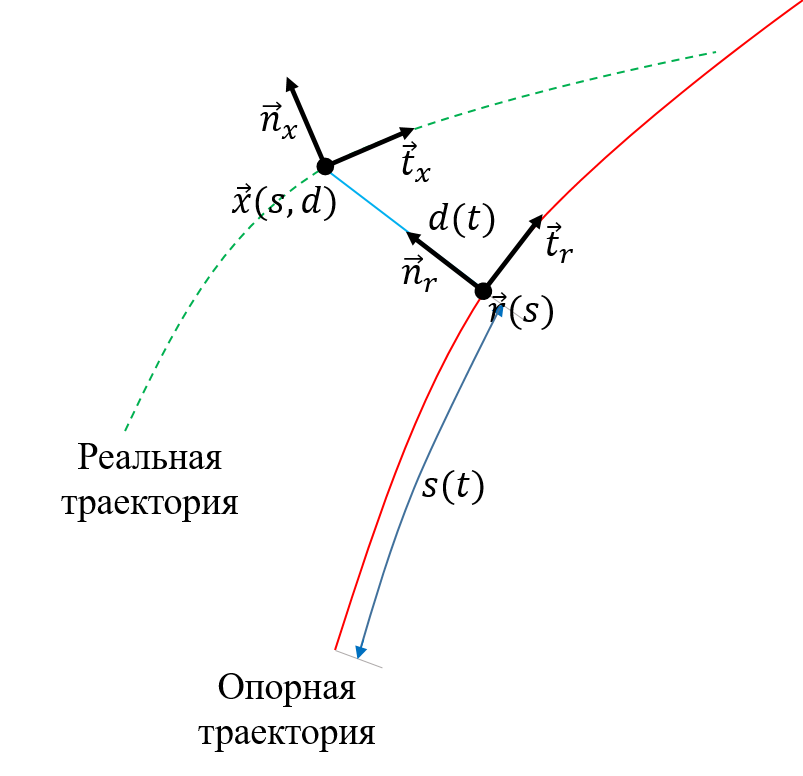
\includegraphics[]{images/frenet_frame}
      \caption{Диаграмма компонентов системы управления беспилотным автомобилем}
      \label{img:frenet_frame}
\end{figure}

Опорная траектория (изображена на рисунке красной линией) представлена натурально параметризованная кривая, где $s(t)$
~--- покрытая длина дуги в момент времени $t$. Положение автомобиля в глобальной системе координат обозначено
радиус-вектором $\vec{x}$. Этому положению автомобиля соответствует подвижная система координат $\vec{r}(s)$,
представляющая собой ортонормированный репер Френе, где $\vec{t}_r$ и $\vec{n}_r$ ~--- касательный и нормальный вектора
к опорной траектории соответственно. Таким образом, положение автомобиля в глобальной декартовой системе кординат
$(x, y)$ может быть представлено в подвижной системе координат как $(s, d)$, где $d$ - расстояние между автомобилем и
опорной траекторией.

Продольная и поперечная траектории движения ищутся в форме полиномов пятого порядка, соединяющие начальное состояние
(текущее состояние автомобиля, полученное от сенсоров) и целевое состояние (полученное от планировщика поведения или
графического интерфейса оператора). Первые и вторые производные этих
полиномов представляют собой зависимость скорости и ускорения автомобиля от времени, которые затем подаются в регулятор
с обратной связью наряду с пространственной траекторией движения, т.е. этот метод позволяет планировать не только
траекторию перемещения автомобиля, но и профиль скорости.

Задача состоит в том чтобы найти коэффициенты полинома, которые минимизируют некую функцию стоимости, используемую для
оценки траекторий. За основу для функции стоимости взят интеграл производной ускорения по времени $\dddot{s}$,
называемая рывок (jerk). Это является распространенным выбором функции стоимости во многих алгоритмов планирования
движения автомобилей. Ниже представлены интегралы для продольного и поперечного движения соответственно:
\begin{equation}
      J_s = \int_{t_0}^{t_1}{\dddot{s}(t)^2dt}
\end{equation}
\begin{equation}
      J_d = \int_{t_0}^{t_1}{\dddot{d}(t)^2dt}
\end{equation}

\noindent\begin{tabularx}{\linewidth}{lllX}
      где & $s(t), d(t)$ &~---& функция продольной и поперечной траекторий соответственно, \\
          & $t_0, t_1$   &~---& начальное и конечное время маневра соответственно. \\
\end{tabularx}

Такой выбор функции стоимости обоснован следующим:
\begin{itemize}
      \item минимизация количества и резкости маневров, совершаемых автомобилем (резкая траектория
            с большим количество маневров может быть получена в результате других алгоритмов
            планирования, таких как RRT), что повышает безопасность и экономичность движения;
      \item обеспечение комфорта пассажиров
\end{itemize}

В соответствии \cite{darpa_junior_frenet_origin} оптимальное решение, минимизирующее рывок, может быть найдено в форме
полиномов пятого порядка:
\begin{eqnarray}
      s(t)        =& a_0t^5   + a_1t^4 + a_2t^3 + a_3t^2 + a_4t + a_5 \\
      \dot{s}(t)  =& 5a_0t^4  + 4a_1t^3 + 3a_2t^2 + 2a_3t + a_4 \\
      \ddot{s}(t) =& 20a_0t^3 + 12a_1t^2 + 6a_2t + 2a_3
\end{eqnarray}

Помимо рывка, функция стоимости должна содержать ряд других членов:
\begin{itemize}
      \item отклонение конечной точки поперечной траектории от опорной траектории ~--- эта функция стоимости
            ухудшает оценку поперечных траекторий, которые не достигают заданной цели;
      \item отклонение конечной точки продольной траектории от покрытой длины дуги целевой точки ~--- эта функция
            стоимости ухудшает оценку продольных траекторий, которые не достигают заданной цели;
      \item отклонение первой производной продольной траектории от требуемой скорости ~--- эта функция стоимости
            ухудшает оценку продольных траекторий, которые не достигают заданной скорости;
      \item общее время совершения маневра ~--- эта функция стоимости ухудшает оценку слишком долгих траекторий.
\end{itemize}

Полная функция стоимости для поперечных траекторий:
\begin{equation}
      C_d = K_{dj} \int_{t_0}^{t_1}{\dddot{d}(t)^2dt} + K_d d(T)^2 + K_{dt} T
\end{equation}

Полная функция стоимости для продольных траекторий:
\begin{equation}
      C_s = K_{sj} \int_{t_0}^{t_1}{\dddot{s}(t)^2dt} + K_s (s(T) - S_1)^2 + K_v (\dot{s}(T) - \dot{S_1}) + K_{st} T
\end{equation}

\noindent\begin{tabularx}{\linewidth}{lllX}
      где & $K_{dj}, K_d, K_{dt}, K_{sj}, K_s, K_v, K_{st}$ &~---& весовые коэффициенты, \\
          & $S_1$                                           &~---& конечное (целевое) продольное состояние, \\
          & $T$                                             &~---& время выполнения маневра. \\
\end{tabularx}

Проблема заключается в том, что при оптимизации коэффициентов полинома необходимо учитывать ограничения. На траекторию
накладываются следующие ограничения:
\begin{itemize}
      \item максимальная продольная скорость,
      \item максимальное продольное ускорение (и замедление),
      \item максимальное поперечное ускорение,
      \item минимальная кривизна траектории,
      \item отсутствие пересечения с препятствиями.
\end{itemize}

Осуществление оптимизации коэффициентов полинома с учетом необходимости проверки на отсутствие пересечений с
препятствиями, которые представлены в виде Occupancy Grid. Поэтому вместо применения методов оптимизации применяется
широко распространенный в задачах планирования движения прием ~--- генерируется большой набор траекторий путем
варьирования конечного состояния $S1(T) = <s(t), \dot{s}(T), \ddot{s}(T)$ и времени $T$ в некотором диапазоне, а затем
производится выбор траектории с наименьшим значением функции стоимости среди тех, которые удовлетворяют ограничениями.

Имея начальное состояние $<s(0), \dot{s}(0), \ddot{s}(0)>$, конечное состояние $<\dot{s}(T), \ddot{s}(T), \ddot{s}(T)>$
и время совершения маневра $T$, можно рассчитать коэффициенты полинома, решив систему уравнений:
\begin{equation}
      \label{eq:solve_quintic}
      \begin{cases}
            \begin{array}
                  {lcl} a_5 = s(0) \\
                        a_4 = \dot{s}(0) \\
                        2a_3 = \ddot{s}(0) \\
                        a_0T^5   + a_1T^4 + a_2T^3 + a_3T^2 + a_4T + a_5 = s(T) \\
                        5a_0T^4  + 4a_1T^3 + 3a_2T^2 + 2a_3T + a_4 = \dot{s}(T)\\
                        20a_0T^3 + 12a_1T^2 + 6a_2T + 2a_3 = \ddot{s}(T)
            \end{array}
      \end{cases}
\end{equation}

На рисунке \ref{img:quntic_example} представлены графики примера продольной траектории, полученные путем решения
системы \ref{eq:solve_quintic}. В этом примере автомобиль тормозит с начальной скорости 15 м/с до полной остановки
за 7 секунд, преодолевая 60 метров.

\begin{figure}[h]
      \centering
      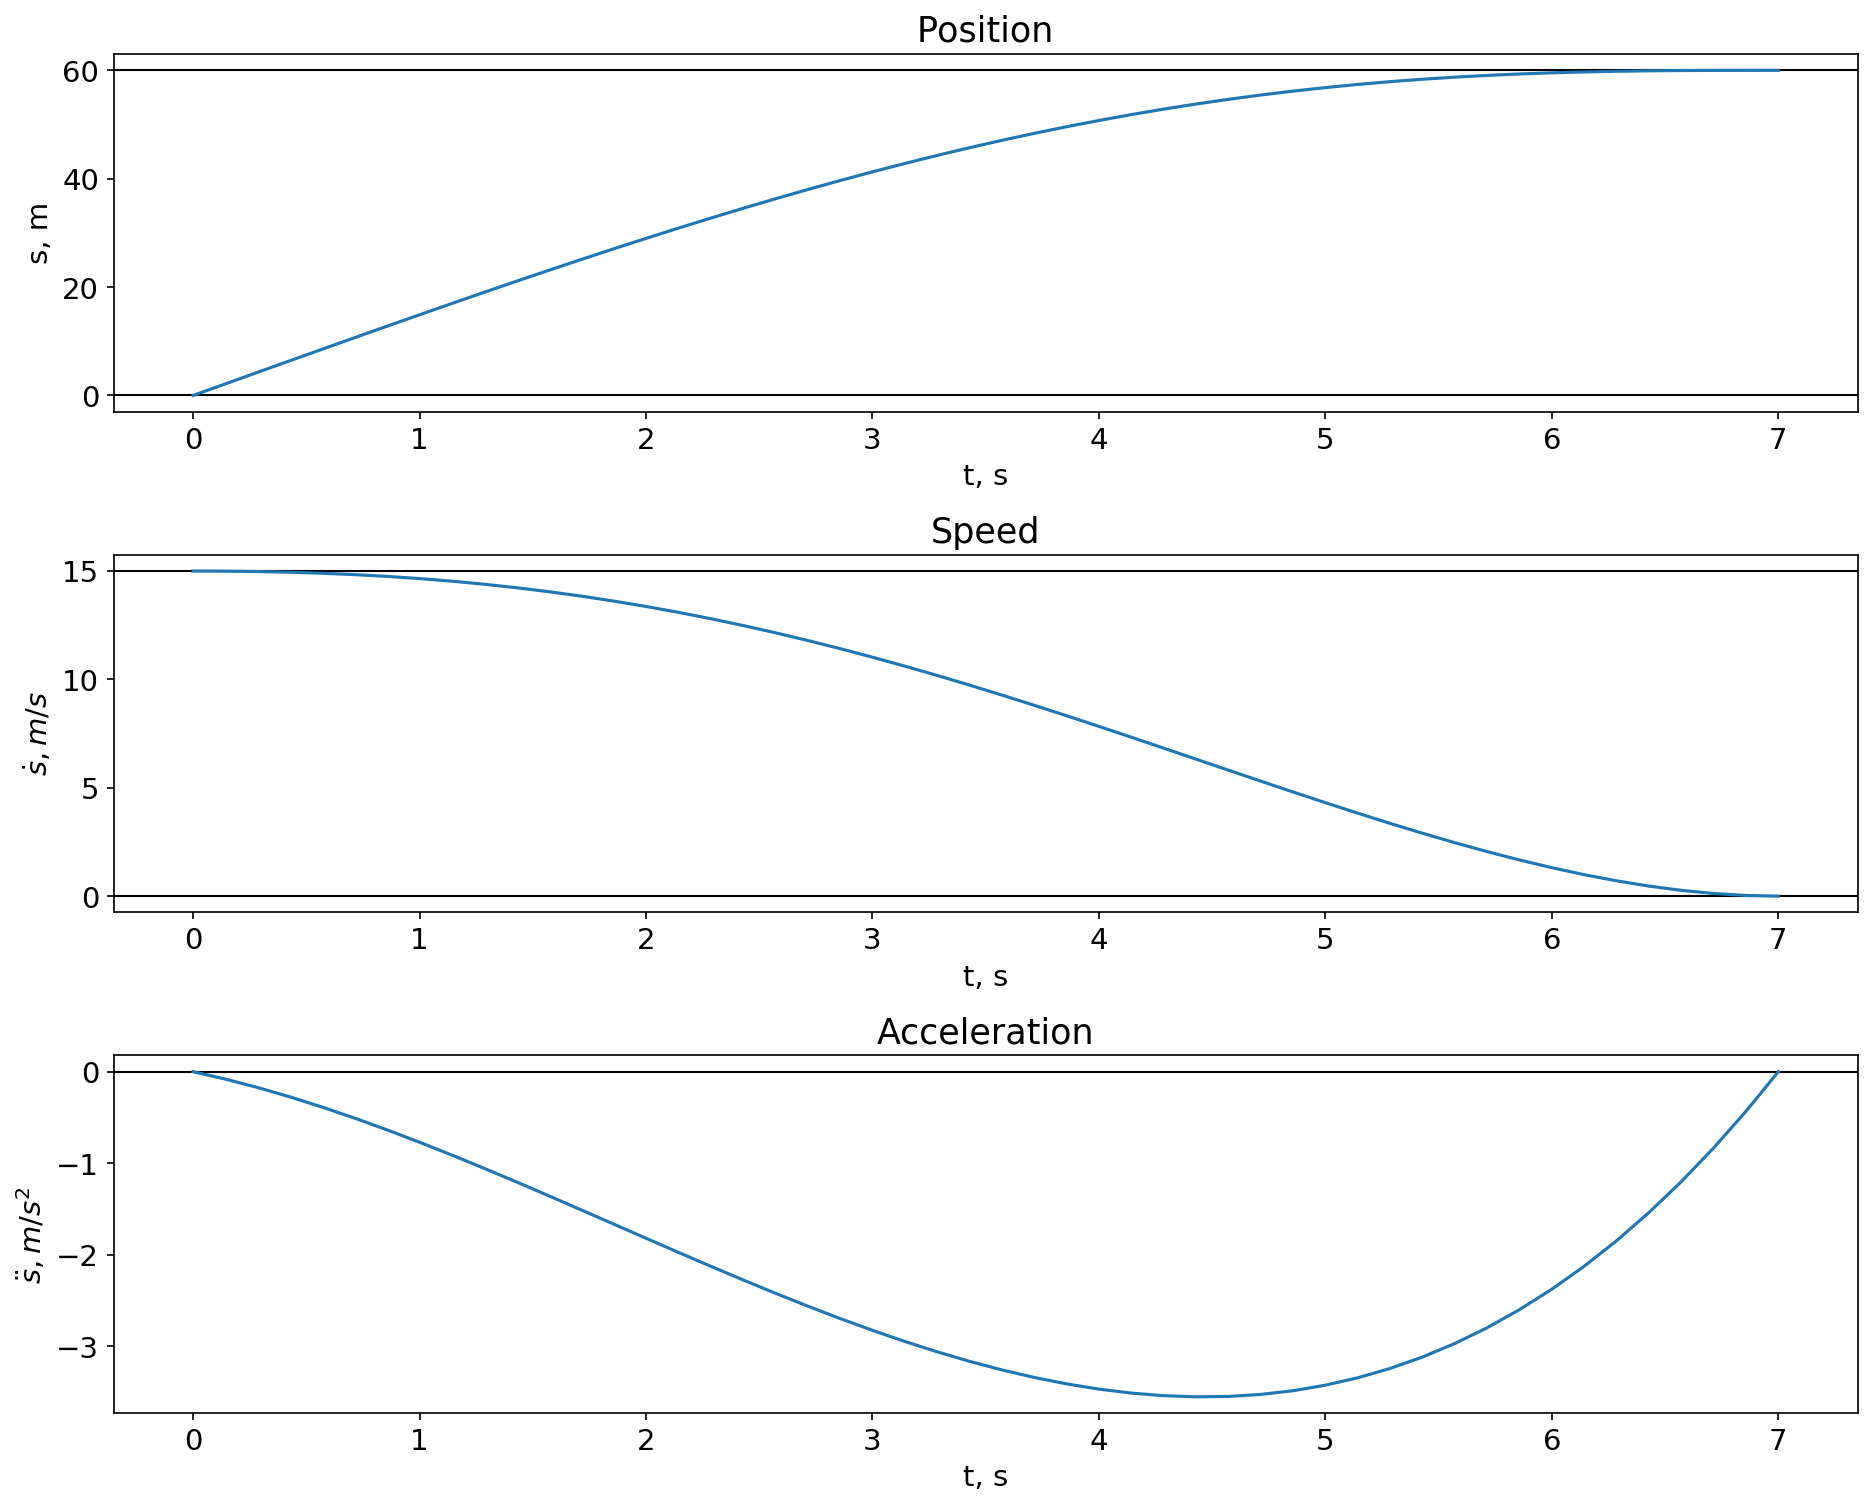
\includegraphics[width=\linewidth]{images/quintic_example}
      \caption{Пример траектории, описываемой полиномом пятого порядка}
      \label{img:quntic_example}
\end{figure}

Набор граничных условий, необходимый для формирования набора траекторий-кандидатов, формируется следующим образом.
Начальное продольное состояние:
\begin{equation}
      S_0 = <s_c, \dot{s}_c, 0>
\end{equation}
\noindent\begin{tabularx}{\linewidth}{lllX}
      где & $s_c$       &~---& текущее положение автомобиля вдоль опорной траектории, полученное от системы SLAM, \\
          & $\dot{s}_c$ &~---& текущая продольная скорость автомобиля, полученная от системы SLAM.
\end{tabularx}

Начальное поперечное состояние:
\begin{equation}
      D_0 = <d_c, \dot{d}_c, 0>
\end{equation}
\noindent\begin{tabularx}{\linewidth}{lllX}
      где & $d_c$       &~---& текущее поперечное отклонение автомобиля от опорной траектории , полученное от системы SLAM, \\
          & $\dot{d}_c$ &~---& скорость изменения поперечного отклонение, полученная от системы SLAM.
\end{tabularx}

Стоит заметить, что поперечная скорость $\dot{d}_c$ в общем случае не является скоростью бокового скольжения автомобиля
и может быть отличной от нуля даже в том случае, если автомобиль движется без бокового скольжения. Если вектор
продольной скорости автомобиля не параллелен касательной к опорной траектории, вектор продольной скорости будет разложен
в пару векторов $\dot{s}_c$ и $\dot{d}_c$.

Конечное продольное состояние:
\begin{equation}
      \begin{aligned}
            S_{1_{ij}} =& <s_i, v_j, 0> \\
            s_i =& s_1 + i\Delta s \\
            v_j =& \dot{s}_1 + i\Delta v
      \end{aligned}
\end{equation}
\noindent\begin{tabularx}{\linewidth}{lllX}
      где & $s_1$       &~---& требуемое положение автомобиля вдоль опорной траектории, получаемое от планировщиков высокого уровня, \\
          & $\dot{s}_1$ &~---& требуемая продольная скорость автомобиля, получаемая от планировщиков выского уровня, \\
          & $\Delta s$  &~---& шаг перебора продольных положений, \\
          & $\Delta v$  &~---& шаг перебора продольных скоростей.
\end{tabularx}

Конечное поперечное состояние:
\begin{equation}
      \begin{aligned}
            D_{1_{ij}} =& <d_i, 0, 0> \\
            d_i =& i\Delta d \\
      \end{aligned}
\end{equation}
\noindent\begin{tabularx}{\linewidth}{lllX}
      где & $\Delta d$  &~---& шаг перебора поперечных положений.
\end{tabularx}

Для перебора конечных состояний поперечных траекторий принимается, что требуемое поперечное положение (отклонение
автомобиля от опорной траектории) всегда равно нулю, т.е. автомобиль должен двигаться ровно по опорной траектории.
В том случае, когда это невозможно, в силу наличия препятствий, или существует более оптимальная траектория (например,
обгон медленно движущегося спереди автомобиля), поперечное движение автомобиля в пределах полосы или выход за ее пределы
осуществляется путем варьирования конечных поперечных состояний в локальном планировщике движения, а не за счет передачи
соответствующих целевых положений планировщиками движения более высокого уровня. Планировщик движения более
высокого уровня, такой как планировщик поведения, может дать команду на смену полосы движения, путем указания
новой опорной траектории, а требуемое  поперечное отклонение от новой траектории по прежнему будет нулевым.

Значения требуемых поперечных скоростей и ускорения полагаются всегда равными нулю, т.е. ожидается, что после завершения
маневра автомобиль будет двигаться параллельно опорной траектории.

Для расчета коэффициентов полинома, описывающего траекторию, требуется определение начального и конечного состояний, как
было описано выше. В качестве начального состояния принимается текущее состояние автомобиля, получаемое от системы
одновременной картографии и навигации (SLAM). Как было сказано выше, система SLAM, позволяет получить текущее положение
$<x, y, z>$ и ориентацию в виде кватерниона углов Эйлера $<\psi, \theta, \varphi>$
\noindent\begin{tabularx}{\linewidth}{lllX}
      где & $\psi$    &~---& рыскание (yaw), вращение вокруг оси $z$, \\
          & $\theta$  &~---& тангаж (pitch), вращение вокруг $y$, \\
          & $\varphi$ &~---& крен (roll), вращение вокруг оси $x$.
\end{tabularx}

Углы Эйлера и соответствующие оси изображены на рисунке \ref{img:euler_angles}.

\begin{figure}[h]
      \centering
      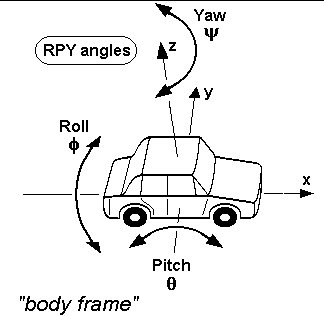
\includegraphics[width=0.5\linewidth]{images/euler_angles}
      \caption{Описание вращения с помощью углов Эйлера}
      \label{img:euler_angles}
\end{figure}

Таким образом, для автомобиля, движущегося на плоскости, состояние может быть задано следующим образом:
$<x, y, \psi, \dot{x}, \dot{y}, \dot{\psi}, \ddot{x}, \ddot{y}, \ddot{\psi}>$. Принимая, что боковое скольжение
отсутствует, состояние автомобиля можно записать в виде $<x, y, \psi, v, \dot{\psi}, a, \ddot{\psi}>$,
где $v$ ~--- продольная скорость, $a$ ~--- продольное ускорение.

Для применения рассматриваемого алгоритма планирования движения, требуется перевести состояние автомобиля из
глобальной декартовой системы координат в подвижную систему координат Френе. \hl{Написать про перевод, либо здесь,
либо в реализации}.

\hl{TODO: написать, что время тоже надо варьировать}

Помимо начального $<s_0, \dot{s}_0, \ddot{s}_0>$, и конечного $<s_1, \dot{s}_1, \ddot{s}_1>$ состояний, для расчета
коэффициентов полинома, согласно \ref{eq:solve_quintic} требуется задать требуемое время маневра $T$. С точки зрения
определения движения автомобиля, явное задание скорости, пройденного расстояния и требуемого для этого времени, является
избыточным. В большинстве случаев требуется монотонное изменение скорости автомобиля (например, ускорение или
замедление). Например, рассмотрим пример, приведенный на рисунке \ref{img:quntic_example}, где автомобиль
ормозит с начальной скорости 15 м/с до полной остановки за 7 секунд, преодолевая 60 метров. Для определения этой траектории
достаточно двух параметров: начальная скорость и требуемый тормозной путь позволяют рассчитать требуемое время, а
начальная скорость и требуемое время до полной остановки позволяют рассчитать требуемый тормозной путь. Существенное
превышение или уменьшение времени маневра $T$ по сравнению с необходимым для совершения этого маневра, не позволит
получить монотонную гладкую траекторию.

На рисунке \ref{img:quntic_bad_t} представлены три траектории:
голубая с близкой к оптимальной длительности маневра, оранжевая со слишком малой длительностью маневра и зеленая, со
слишком большой длительностью маневра. Видно, что при оптимальной длительности маневра положение автомобиля монотонно
возрастает, а скорость ~--- монотонно убывает. При слишком малой длительности маневра первоначально происходит
ускорение и лишь потом замедление до требуемой скорости. При слишком большой длительности маневра автомобиль сначала
проезжает мимо целевого положения, а затем возвращается, т.е. имеете место участок с отрицательной скоростью
(движение назад).

\begin{figure}[h]
      \centering
      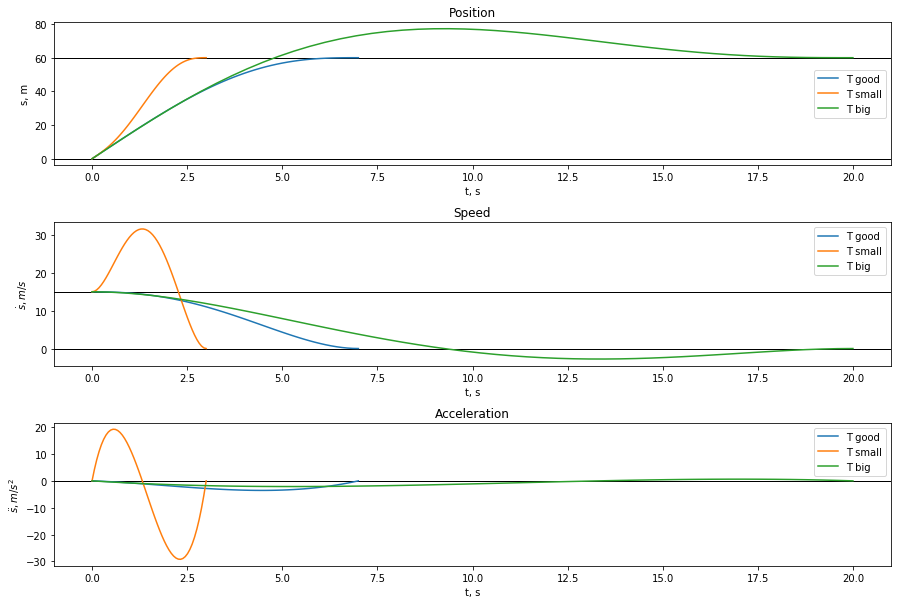
\includegraphics[width=\linewidth]{images/quintic_bad_t}
      \caption{Зависимость траектории от времени совершения маневра}
      \label{img:quntic_bad_t}
\end{figure}

Варьирование времени маневра $T$ может быть применено для получения различных профилей скорости. Так, например,
первоначальное ускорение с последующим замедлением может быть использовано при маневрах обгона.
В работе \cite{darpa_boss}, посвященной автомобилю "BOSS" Darpa Urban Challenge применяются несколько явно заданных
профилей скорости. С одной стороны, явное параметрическое задание профиля скорости позволяет более точно и задавать
требуемый профиль скорости и иметь большее число вариантов профиля скорости, в отличие от примененного в этой работе
метода, в котором профиль скорости задается неявно путем варьирования одного параметра ~--- длительности маневра $T$.
С другой стороны, метод, применяемый в автомобиле BOSS, обладает следующим недостатком: форма траектории и профиль
скорости выбираются независимо, в то время как в методе, реализуемым  в данной работе, профили скорости и ускорения
являются производными траектории, таким образом, этот метод лучше учитывает динамические характеристики автомобиля.

Таким образом, аналогично с варьированием конечных состояний, требуется варьировать длительность маневра:
\begin{equation}
      T_k = T_e + k\Delta T
\end{equation}
\noindent\begin{tabularx}{\linewidth}{lllX}
      где & $T_e$      &~---& начальная оценка длительности маневра, \\
          & $\Delta T$ &~---& шаг перебора длительностей маневра.
\end{tabularx}

Можно было бы задать в качестве начальной оценки заранее определенное константное значение времени либо перебирать
все значения от 0 до некого заданного $T_{max}$. Но это было бы неоптимально, потому что в таком случае было бы
сгенерировано большое количество траекторий со слишком малой или слишком большой длительностью маневра. Эти траектории
не повлияют на итоговый результат планирования движения, т.к. в любом случае будет выбираться оптимальная траектория,
минимизирующая функционал стоимости, но расчет большого количества избыточных траекторий серьезно увеличит вычислительные
затраты и время работы алгоритма.

Чтобы избежать этого был предложен метод приблизительной оценки требуемой длительности маневра $T_e$. В качестве оценки
требуемого времени совершения маневра принимается время совершения маневра с такими же начальными и конечными
условиями, но для случая равноускоренного движения:
\begin{equation}
      \begin{cases}
            \dot{s}_1 = \dot{s}_0 + aT_e \\
            s_1       = s_0       + \dot{s}_0T_e + \frac{aT_e^2}{2}
      \end{cases}
\end{equation}

Решая эту систему получим формулу расчет оценки времени маневра:
\begin{equation}
      T_e = 2\frac{s_0 - s_1}{\dot{s}_0 + \dot{s}_1}
\end{equation}

На рисунке \ref{img:quintic_t_estimate} приведен пример оценки длительности маневра.

\begin{figure}[h]
      \centering
      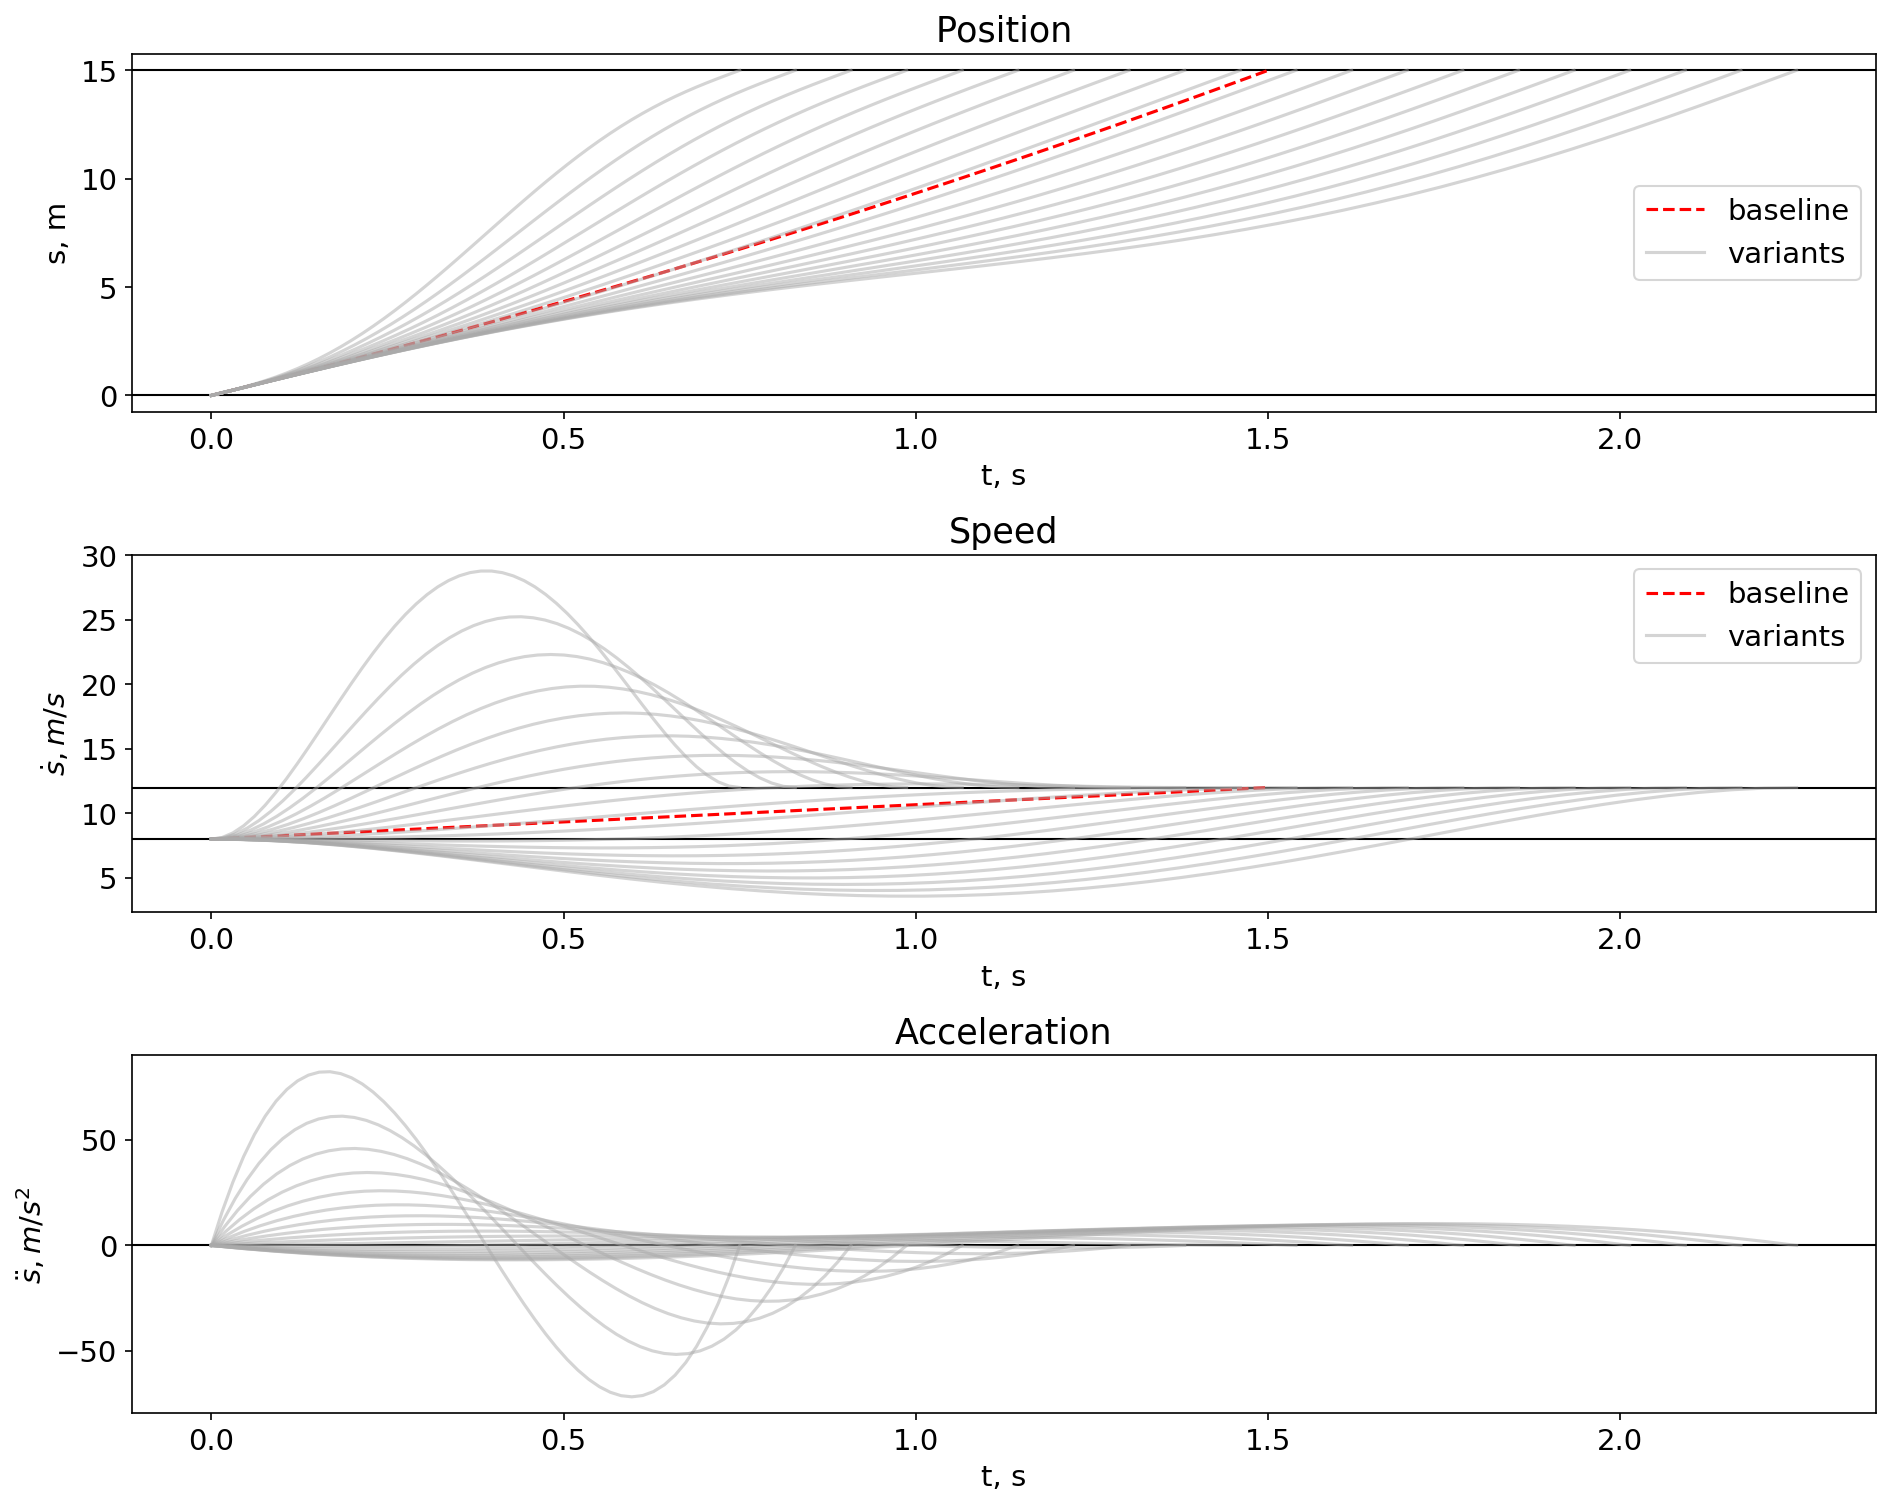
\includegraphics[width=\linewidth]{images/quintic_t_estimate}
      \caption{Пример оценки длительности маневра с помощью равноускоренного движения. Пунктирная линия ~---
      траектория равноускоренного движения, сплошные линии - траектории, полученные путем варьирования длительности
      маневра при одинаковых начальных и конечных условиях.}
      \label{img:quintic_t_estimate}
\end{figure}

\subsection{???}


\section{Проектирование подсистемы следования траектории}
